\documentclass[9pt]{article}
% Smaller margins using geometry
\usepackage[a4paper, margin=1in]{geometry} % Try margin=0.75in for even tighter layout

\usepackage[english]{babel}
\usepackage[utf8x]{inputenc}
\usepackage[T1]{fontenc}
\usepackage{setspace}
\usepackage{lmodern}
\usepackage{microtype}

\usepackage{amsmath}
\usepackage{steinmetz}
\usepackage{listings}

\usepackage{comment}
\usepackage{upgreek}

\usepackage{siunitx}
\sisetup{exponent-product = \cdot}
\DeclareSIUnit\epoch{epoch}
\usepackage{nicefrac}
\usepackage{multirow}
\usepackage{booktabs}

\usepackage{graphicx}
\usepackage{float}
\usepackage{pgfplots}
\usepackage{pgfplotstable}
\pgfplotsset{compat=1.16}

\usepackage{caption}
\captionsetup[table]{position=bottom}
\usepackage{subcaption}
\usepackage{csvsimple}

\usepackage{tablefootnote}

\usepackage[hidelinks]{hyperref}
\usepackage{cleveref}
\crefformat{section}{#2\S#1#3}
\Crefname{figure}{Fig.}{Fig.}

\newcommand{\placeholder}{\textcolor{red}{[PLACEHOLDER]~}}
\newcommand{\todo}{\textcolor{red}{[TODO]:~}}

% reduce space between paragraphs
\makeatletter
\renewcommand\paragraph{\@startsection{paragraph}{4}{\z@}%
                                    {1.5ex \@plus1ex \@minus.2ex}%
                                    {-1em}%
                                    {\normalfont\normalsize\bfseries}}
\makeatother

\title{Project 4: Natural Language Processing\\Group 2}

\author{Chiara Iorio - s343732, Renato Mignone - s336973, \\ Claudia Sanna - s343470}
\date{}

\begin{document}

\maketitle
\renewcommand{\abstractname}{\vspace{-\baselineskip}}
\vspace{-15pt}
\begin{abstract}
\noindent The goal of this laboratory is to apply Natural Language Processing (NLP) techniques in the context of cybersecurity. Specifically, we will analyze a dataset consisting of SSH sessions, represented as sequences of SSH entities, such as commands, flags, parameters, and separators. We will perform dataset characterization, then we will analyze the impact of different tokenization strategies and experiment with various pre-trained Language Models, comparing their performance. Finally, we will use the fine-tuned model for inference to investigate cybersecurity threats and infer the intentions of potentially malicious users.
\end{abstract}


\section{Dataset Characterization}
In this section, we explore the provided training and test datasets.

\paragraph{Labels exploration} \Cref{fig:task1_ecdf_bash_words} illustrates the distribution of tags in both the training and test sets. The datasets comprise seven distinct tags: \emph{Defense Evasion}, \emph{Discovery}, \emph{Execution}, \emph{Impact}, \emph{Not Malicious Yet}, \emph{Other}, and \emph{Persistence}. Generally, the number of Bash words assigned to a tag is higher in the training set than in the test set. In fact, the training set contains 11475 Bash words distributed among 251 sessions, while the test set only 6197 (108 sessions). Both sets exhibit a similar distribution profile: \emph{Discovery} ($\approx\SI{50}{\percent}$) is the most prevalent tag, followed by \emph{Execution} ($\approx\SI{25}{\percent}$), and \emph{Persistence} ($\approx\SI{10}{\percent}$). The remaining four tags are significantly less frequent, each appearing in less than \SI{4}{\percent} instances.

\paragraph{The \texttt{echo} command} The \texttt{echo} command has been assigned to 6 different tags: \emph{Persistence} (104 times), \emph{Execution} (39 times), \emph{Discovery} (31 times), \emph{Not Malicious Yet} (8 times), \emph{Impact} (6 times), and \emph{Other} (4 times). We will now analyze two example of sessions: one in which \texttt{echo} is labelled as \emph{Persistence} and one as \emph{Execution}.

\textbf{(\texttt{echo}, Persistence):} \texttt{[\dots]; echo ``root:HGbB4i9gUXMh' | chpasswd | bash ; [\dots]}. The \texttt{echo} outputs the string \texttt{root:HGbB4i9gUXMh} (username:password hash), which is piped to \texttt{chpasswd}, that updates user passwords from standard input. By changing the \texttt{root} user's password to a known value, the attacker gains persistent administrative access to the compromised system.

\textbf{(\texttt{echo}, Execution):} \texttt{[\dots]; echo
``base64\_payload'' | base64 --decode | bash ;}. The \texttt{echo} outputs a base64 payload, that is then decoded and executed. Hence, the command immediately executes arbitrary code, probably a malware binary.

In both cases, the \texttt{echo} command is used to output a string. However, the meaning of this string and the goal of the subsequent commands influence the labelling of \texttt{echo} itself: \emph{Persistence} in the first case, and \emph{Execution} in the second one.

\paragraph{Bash words exploration} \Cref{fig:task1_ecdf_bash_words} shows the ECDF of Bash words per session in both the training and test sets. The distribution shows that most sessions are relatively short, with \SI{50}{\percent} containing less than 25 words, and $\approx\SI{80}{\percent}$ less than 100 words. While both datasets share the same minimum (2 words) and maximum (224 words) lengths, the test set is generally characterized by longer sessions. Specifically, the mean session length in the test set is \SI{57.38}{\words}, compared to \SI{45.70}{\words} in the training set. This right-skewed distribution indicates the presence of a few longer sessions that contrast with the high frequency of shorter ones.

\begin{figure}
	\centering
    \subfloat[][{Tag distribution.}\label{fig:task1_tags_distribution}]
	{\includegraphics[width=.54\linewidth]{img/Task1/task1_tags_distribution.png}} \quad
	\subfloat[][{ECDF of Bash words per session.}\label{fig:task1_ecdf_bash_words}]
	{\includegraphics[width=.429\linewidth]{img/Task1/task1_ecdf_length.png}} \\
  	\caption{Plots about Dataset Characterization. Both plots refer to the training and test sets.}{}\label{fig:task1}
\end{figure}
\section{Tokenization}
In this section, we compare the tokenization behavior of two pre-trained tokenizers: BERT (google-bert/bert-base-uncased), a general-purpose model trained on English text, and UniXcoder (microsoft/unixcoder-base), a code-oriented model designed for programming languages.

\paragraph{Command tokenization} We first tokenize a sample list of SSH commands: \texttt{cat}, \texttt{shell}, \texttt{echo}, \texttt{top}, \texttt{chpasswd}, \texttt{crontab}, \texttt{wget}, \texttt{busybox}, and \texttt{grep}. The BERT tokenizer divides words into subword units based on frequency in general English text, while the UniXcoder tokenizer understands common shell commands and structures from its code-centric training. Both tokenizers keep certain words intact because they represent high-frequency tokens in their training data. For instance, \texttt{cat}, \texttt{echo}, and \texttt{grep} are common enough to have dedicated vocabulary entries. UniXcoder has many bash commands in its vocabulary from code training, while BERT retains them only if they appear frequently in general text.

\paragraph{Full corpus tokenization} When tokenizing the entire training corpus, BERT produces on average \SI{178.6}{\tokens} per session with a maximum of \SI{1889}{\tokens}, while UniXcoder produces on average \SI{409.3}{\tokens} per session with a maximum of \SI{28920}{\tokens}. UniXcoder tends to generate more tokens because it performs code-specific splitting on characters like \texttt{\{}, \texttt{\&\&}, and handles file paths differently. \Cref{fig:task2_ecdf_tokens} shows the ECDF distribution of token counts. The vertical red line marks the 512-token context size limit of both models.

\begin{figure}
	\centering
    \subfloat[][{ECDF for BERT.}\label{fig:task2_ecdf_bert}]
	{\includegraphics[width=.48\linewidth]{img/Task2/ecdf_distribution_tokens_bert.png}} \quad
	\subfloat[][{ECDF for UniXcoder.}\label{fig:task2_ecdf_unixcoder}]
	{\includegraphics[width=.48\linewidth]{img/Task2/ecdf_distribution_tokens_unixcode.png}} \\
  	\caption{ECDF distribution of number of tokens per session for both tokenizers. The red line indicates the model context size (512 tokens).}\label{fig:task2_ecdf_tokens}
\end{figure}

\paragraph{Truncation analysis} With the 512-token limit, 24 sessions would be truncated by the BERT tokenizer and 29 by the UniXcoder tokenizer. The longest session contains 224 words, but produces 1889 tokens with BERT and 28920 with UniXcoder. In the BERT-tokenized version, 113 tokens are marked as \texttt{[UNK]} (unknown), while UniXcoder produces 0 unknown tokens, demonstrating its superior handling of code-specific vocabulary.

\paragraph{Word truncation preprocessing} Since \SI{98}{\percent} of words are shorter than 30 characters, we truncate all words exceeding this length before tokenization. After this preprocessing step, token counts decrease significantly: BERT produces on average \SI{128}{\tokens} per session (max 613), while UniXcoder produces on average \SI{111}{\tokens} per session (max 540). This reduces the number of truncated sessions to only 6 for both tokenizers.

The token-to-word ratios after preprocessing are 2.79 for BERT and 2.43 for UniXcoder. UniXcoder achieves the better (lower) ratio, indicating more efficient tokenization for this domain. \Cref{fig:task2_words_vs_tokens} shows the relationship between the number of words and tokens per session for both tokenizers, highlighting UniXcoder's more compact representation.

\begin{figure}
	\centering
    \subfloat[][{BERT.}\label{fig:task2_words_bert}]
	{\includegraphics[width=.48\linewidth]{img/Task2/number_words_vs_number_tokens_bert.png}} \quad
	\subfloat[][{UniXcoder.}\label{fig:task2_words_unixcoder}]
	{\includegraphics[width=.48\linewidth]{img/Task2/number_words_vs_number_tokens_unixcoder.png}} \\
  	\caption{Number of words vs number of tokens per session after word truncation at 30 characters.}\label{fig:task2_words_vs_tokens}
\end{figure}
\section{Model training}\label{sec:task3}
In this section, we train and compare different transformer-based models for token-level classification of SSH sessions into MITRE tactics. We evaluate: (1)~pre-trained BERT, (2)~randomly initialized (naked) BERT, (3)~pre-trained UniXcoder, and (4)~alternative fine-tuning strategies with frozen layers. For each configuration, we perform a grid search over learning rates and select the best model based on the validation loss and macro F1-score on the validation loss. Specifically, the validation loss allows detecting divergence or instability typical of overfitting, while validation macro F1-score better reflects classification performance. We split the training set into \SI{80}{\percent} training and \SI{20}{\percent} validation, using the provided test set for the final evaluation.

\subsection{Fine-tuning Pre-trained BERT}
\paragraph{Model selection} First, we fine-tune a pre-trained BERT model for Named Entity Recognition, using the pre-trained weights. We trained the model for 40 epochs and with three different learning rates (\num{5e-6}, \num{1e-5} and \num{2e-5}). \Cref{fig:task3_bert_results} shows the validation loss and macro F1-score curves for different learning rates: the \num{1e-5} learning rate achieves the best balance between convergence speed and final performance, with validation loss stabilizing around epoch 20 and macro F1-score reaching its peak of \num{0.60}. While the higher learning rate (\num{2e-5}) reached a comparable F1-score more quickly (by epoch 12), it also exhibited immediate signs of overfitting thereafter. With a lower learning rate (\num{5e-6}), the model converges slower and achieves a significantly lower macro F1-score. Consequently, we selected the model trained with learning rate \num{1e-5} to prioritize validation stability over the slightly faster, but more volatile, convergence of higher learning rates, and implemented manual early stopping at epoch 20.

\paragraph{Performance evaluation} The performance on the test set is summarized in \cref{tab:task3_comparison}. Despite being trained on only 251 labeled sessions, the model achieves competitive token-level accuracy (\num{0.87}) and macro F1-score (\num{0.64}), indicating effective knowledge transfer from pre-training. The recall-precision imbalance (\num{0.57} vs {0.84}) indicates that the model is conservative, generating more false negatives than false positives. The average session fidelity is \num{0.82}, meaning that, in general, the model correctly predicts four fifths of tokens in each session. Analyzing the per-class F1 scores (\cref{fig:task3_f1_comparison}), we observe that the model performs well on high-support classes (\emph{Discovery}: \num{0.91}, \emph{Execution}: \num{0.87}, \emph{Persistence}: \num{0.92}) but struggles with minority classes (\emph{Defense Evasion}: 0.40, \emph{Other}: \num{0.34}).


\begin{figure}
	\centering
    \subfloat[][{Validation loss.}\label{fig:task3_bert_val}]
	{\includegraphics[width=.48\linewidth]{img/Task3/task3_bert_fine_tuned_val_loss.png}} \quad
	\subfloat[][{Validation macro F1-score.}\label{fig:task3_bert_f1_curve}]
	{\includegraphics[width=.48\linewidth]{img/Task3/task3_bert_fine_tuned_val_macro_f1_scores.png}} \\
  	\caption{Validation curves for pre-trained BERT with different learning rates.}\label{fig:task3_bert_results}
\end{figure}

\subsection{Naked BERT Baseline}
\paragraph{Model selection} To verify that pre-training is essential, we train a naked BERT model from scratch, meaning that we use the same architecture of the previous case, but initialized with random weights. We train the model for 40 epochs and with three different learning rates (\num{5e-6}, \num{1e-5}, \num{5e-5}). Following the same approach previously used, we select the configuration with 25 epochs and learning rate \num{5e-5}, since it achieves the best validation loss and macro F1-score among the experimented configurations.

\paragraph{Performance evaluation} \Cref{tab:task3_comparison} compares the results between the pre-trained BERT model and the naked one. The naked BERT achieves only \SI{74.02}{\percent} token accuracy, a drop of nearly 13 percentage points compared to the pre-trained version. Also macro precision, recall and F1-score are significantly lower than in the previous case, while the average session fidelity is only slightly worse (\num{0.77} vs \num{0.83}). Moreover, \cref{fig:task3_f1_comparison} shows that naked BERT achieves a lower F1-score in all classes compared to the fine-tuned model.  This confirms that SSH command classification is not trivial: the 251 training samples are insufficient for learning from scratch, and pre-trained weights provide essential baseline knowledge that the naked model cannot discover with such limited data.

\subsection{Fine-tuning UniXcoder}
\paragraph{Model selection} Since UniXcoder was pre-trained on a large code corpus, we hypothesize it has more relevant prior knowledge for SSH command analysis. To find the best learning rate and number of epochs, we performed a grid search over learning rates \num{5e-6}, \num{1e-5}, \num{4e-5}, training all models for 40 epochs. \Cref{fig:task3_unixcoder_results} shows the validation loss and macro F1-score curves: the \num{1e-5} learning rate achieves stable convergence with validation loss decreasing smoothly and macro F1-score reaching $\approx\num{0.65}$, outperforming all BERT configurations. Consequently, we selected the model trained with \num{1e-5} to prioritize validation stability over the more volatile convergence of higher learning rates, anyway leading to similar performance. Moreover, we implemented manual early stopping at epoch 15 to prevent overfitting.

\paragraph{Performance evaluation} \Cref{tab:task3_comparison} summarizes the results achieved by the model on the test set. The hypothesis is confirmed: UniXcoder achieves \SI{89.01}{\percent} token accuracy, outperforming pre-trained BERT by over 2 percentage points. The macro F1-score improves from \num{0.64} to \num{0.69} ($+\num{0.05}$). While UniXcoder achieves a slightly lower token precision ($-\SI{0.43}{\percent}$), the recall increases by \SI{5.2}{\percent} with respect to pre-trained BERT. UniXcoder's specialized vocabulary and representations learned from code corpora enable better handling of shell syntax, operators, and path structures. As shown in \cref{fig:task3_f1_comparison}, UniXcoder is significantly better at identifying \emph{Defense Evasion} samples (F1-score \num{0.76} vs \num{0.40} for pre-trained BERT), likely because code pre-training helps recognize obfuscation patterns; instead UniXcoder only performs similarly to pre-trained BERT on the other tags.

\begin{table}
\small
\centering
\caption{Comparison of token classification metrics between all models on the test set. Precision, Recall, and F1-score are computed using macro-averaging.}
\label{tab:task3_comparison}
\begin{tabular}{lccccc}
\toprule
Model & Accuracy & Precision & Recall & F1-score & Avg Fidelity \\
\midrule
Pre-trained BERT  		& 0.8694 & 0.8402 & 0.5746 & 0.6399 & 0.8267 \\
Naked BERT        		& 0.7402 & 0.5469 & 0.4775 & 0.4925 & 0.7701 \\
UniXcoder (Full)  		& 0.8901 & 0.8359 & 0.6265 & 0.6909 & 0.8411 \\
UniXcoder (Last 2 + Head)  	& 0.8714 & 0.8043 & 0.5972 & 0.6521 & 0.8294 \\
UniXcoder (Head Only) 	& 0.8035 & 0.7206 & 0.5093 & 0.5628 & 0.7527 \\
\bottomrule
\end{tabular}
\end{table}

\begin{table}
\small
\centering
\caption{Comparison of the number of parameters and training time using different fine-tuning strategies for UniXcoder.}
\label{tab:task3_alternative}
\begin{tabular}{lS[table-format=9.0, group-minimum-digits = 4]S[table-format=3.3]
c}
\toprule
Configuration & {Trainable Parameters} & {\si{\percent} Trainable Parameters} & Time/epoch \\
\midrule
Full fine-tuning       & 125344519 & 100.000  & \SI{4.5}{\second} \\
Last 2 Layers + Head  & 14181127 & 11.310 & \SI{2.0}{\second} \\
Head Only          & 5383 & 0.004  & \SI{1.5}{\second} \\
\bottomrule
\end{tabular}
\end{table}

\begin{figure}
	\centering
	\includegraphics[width=0.98\linewidth]{img/Task3/bert_unixcoder_barplot.png}
	\caption{Per-class F1 scores on the test set for all model configurations.}
	\label{fig:task3_f1_comparison}
\end{figure}

\begin{figure}
	\centering
    \subfloat[][{Validation loss.}\label{fig:task3_unix_val}]
	{\includegraphics[width=.48\linewidth]{img/Task3/task3_unixcoder_fine_tuned_val_loss.png}} \quad
	\subfloat[][{Validation macro F1-score.}\label{fig:task3_unix_f1_curve}]
	{\includegraphics[width=.48\linewidth]{img/Task3/task3_unixcoder_fine_tuned_val_macro_f1_scores.png}} \\
  	\caption{Validation curves for UniXcoder with different learning rates.}\label{fig:task3_unixcoder_results}
\end{figure}

\subsection{Alternative Fine-tuning Strategies}
We explore parameter-efficient fine-tuning by freezing portions of the UniXcoder model, that, as analyzed in the previous paragraphs, it is the best performing one. We test two configurations: (1)~training only the last 2 encoder layers + classification head, and (2)~training only the classification head.

\paragraph{Model Selection} To find the best learning rate and number of epochs, we performed a grid search over learning rates \num{1e-5}, \num{5e-5}, \num{7.5e-5} for the fine-tuning of the last two encoding layers + classification head and \num{1e-4}, \num{5e-4}, \num{1e-3} for the fine-tuning of the classification head, training all models for 40 epochs. Given the validation loss curves and the validation macro F1-score, we select learning rate \num{5e-5} and 20 epochs for the first model, and \num{1e-3} and 10 epochs for the second one.

\paragraph{Strategies comparison} \Cref{tab:task3_alternative} summarizes the number of parameters and training time\footnote{Executed on Google Colab, Runtime with T4 GPU} using different fine-tuning strategies for UniXcoder. The full fine-tuning trains all 125.3M parameters, ``Last 2 Layers + Head'' trains 14.18M parameters (\SI{11.31}{\percent}), and ``Head Only'' trains only 5.38k parameters (\SI{0.004}{\percent}). Consequently, reducing the number of parameters to train also leads to a reduction in the training time: in the  ``Last 2 Layers + Head'' configuration the time to complete each epoch is less than half compared to that of the full fine-tuning scenario (\SI{2.0}{\second} vs \SI{4.5}{\second}). In the ``Head Only'' this time is even smaller (\SI{1.5}{\second}).

When fine-tuning only the final layers of the UniXcoder model, we observed that a higher learning rate is necessary to achieve optimal convergence, especially in the ``Head Only'' case.  While full fine-tuning typically utilizes a smaller learning rate to preserve pre-trained knowledge across the entire architecture, partial fine-tuning requires a more aggressive approach in the unfrozen layers to effectively map those fixed features to the target labels within a reasonable number of epochs.

\paragraph{Performance evaluation} \Cref{tab:task3_comparison} summarizes the test set results. Full fine-tuning achieves the highest results. The ``Last 2 Layers + Head'' fine-tuning shows a drop of less than \SI{3}{\percent} on most metrics, demonstrating that freezing most layers still yields competitive results, while reducing the training time. The ``Head Only'' fine-tuning, instead, achieves considerably lower results, with a \SIrange[range-units = single, range-phrase = \,--\,]{7}{10}{\percent} decrease in respect to the full fine-tuned case, showing that this approach fails to properly learn fundamental discriminative patterns.

\Cref{fig:task3_f1_comparison} provides a comparison of per-class F1 scores across the different configurations. UniXcoder (Full) consistently outperforms both alternative fine-tuning strategies. Progressive freezing degrades performance proportionally: ``Last 2 Layers + Head'' maintains competitive scores on majority classes but drops on \emph{Defense Evasion} (\num{0.59} vs \num{0.76}) and \emph{Impact} (\num{0.39} vs \num{0.50}). Interestingly, it performs better on the \emph{Other} tag (\num{0.45} vs \num{0.34}).  ``Head Only'' performs significantly worse than the other models, particularly on \emph{Not Malicious Yet} (0.29), confirming that adapting encoder representations is essential for recognizing obfuscation patterns. While the fine-tuned BERT model generally performs better than ``Last 2 Layers + Head'' and ``Head Only'', naked BERT is consistently outperformed by all UniXcoder models, demonstrating the importance of pre-training on context specific knowledge.

\subsection{Summary and Best Model Selection}
From the results summarized in \cref{tab:task3_comparison}, it is evident that the best performance is achieved by the fully fine-tuned UniXcoder. Even though the ``Last 2 Layers + Head'' model achieves competitive results with a more time-efficient training, we decided to use the fully fine-tuned model for the inference task discussed in \cref{sec:task4} since we only train the model for 15 epochs and thus the training time difference is negligible.
\section{Inference}
"On the other hand, \cref{fig:architectureschema} we denounce with righteous indignation and dislike men who are so beguiled and demoralized by the charms of pleasure of the moment, so blinded by desire, that they cannot foresee the pain and trouble that are bound to ensue; and equal blame belongs to those who fail in their duty through weakness of will, which is the same as saying through shrinking from toil and pain. These cases are perfectly simple and easy to distinguish. In a free hour, when our power of choice is untrammelled and when nothing prevents our being able to do what we like best, every pleasure is to be welcomed and every pain avoided. But in certain circumstances and owing to the claims of duty or the obligations of business it will frequently occur that pleasures have to be repudiated and annoyances accepted. The wise man therefore always holds in these matters to this principle of selection: he rejects pleasures to secure other greater pleasures, or else he endures pains to avoid worse pains."

\begin{figure}
	\centering
	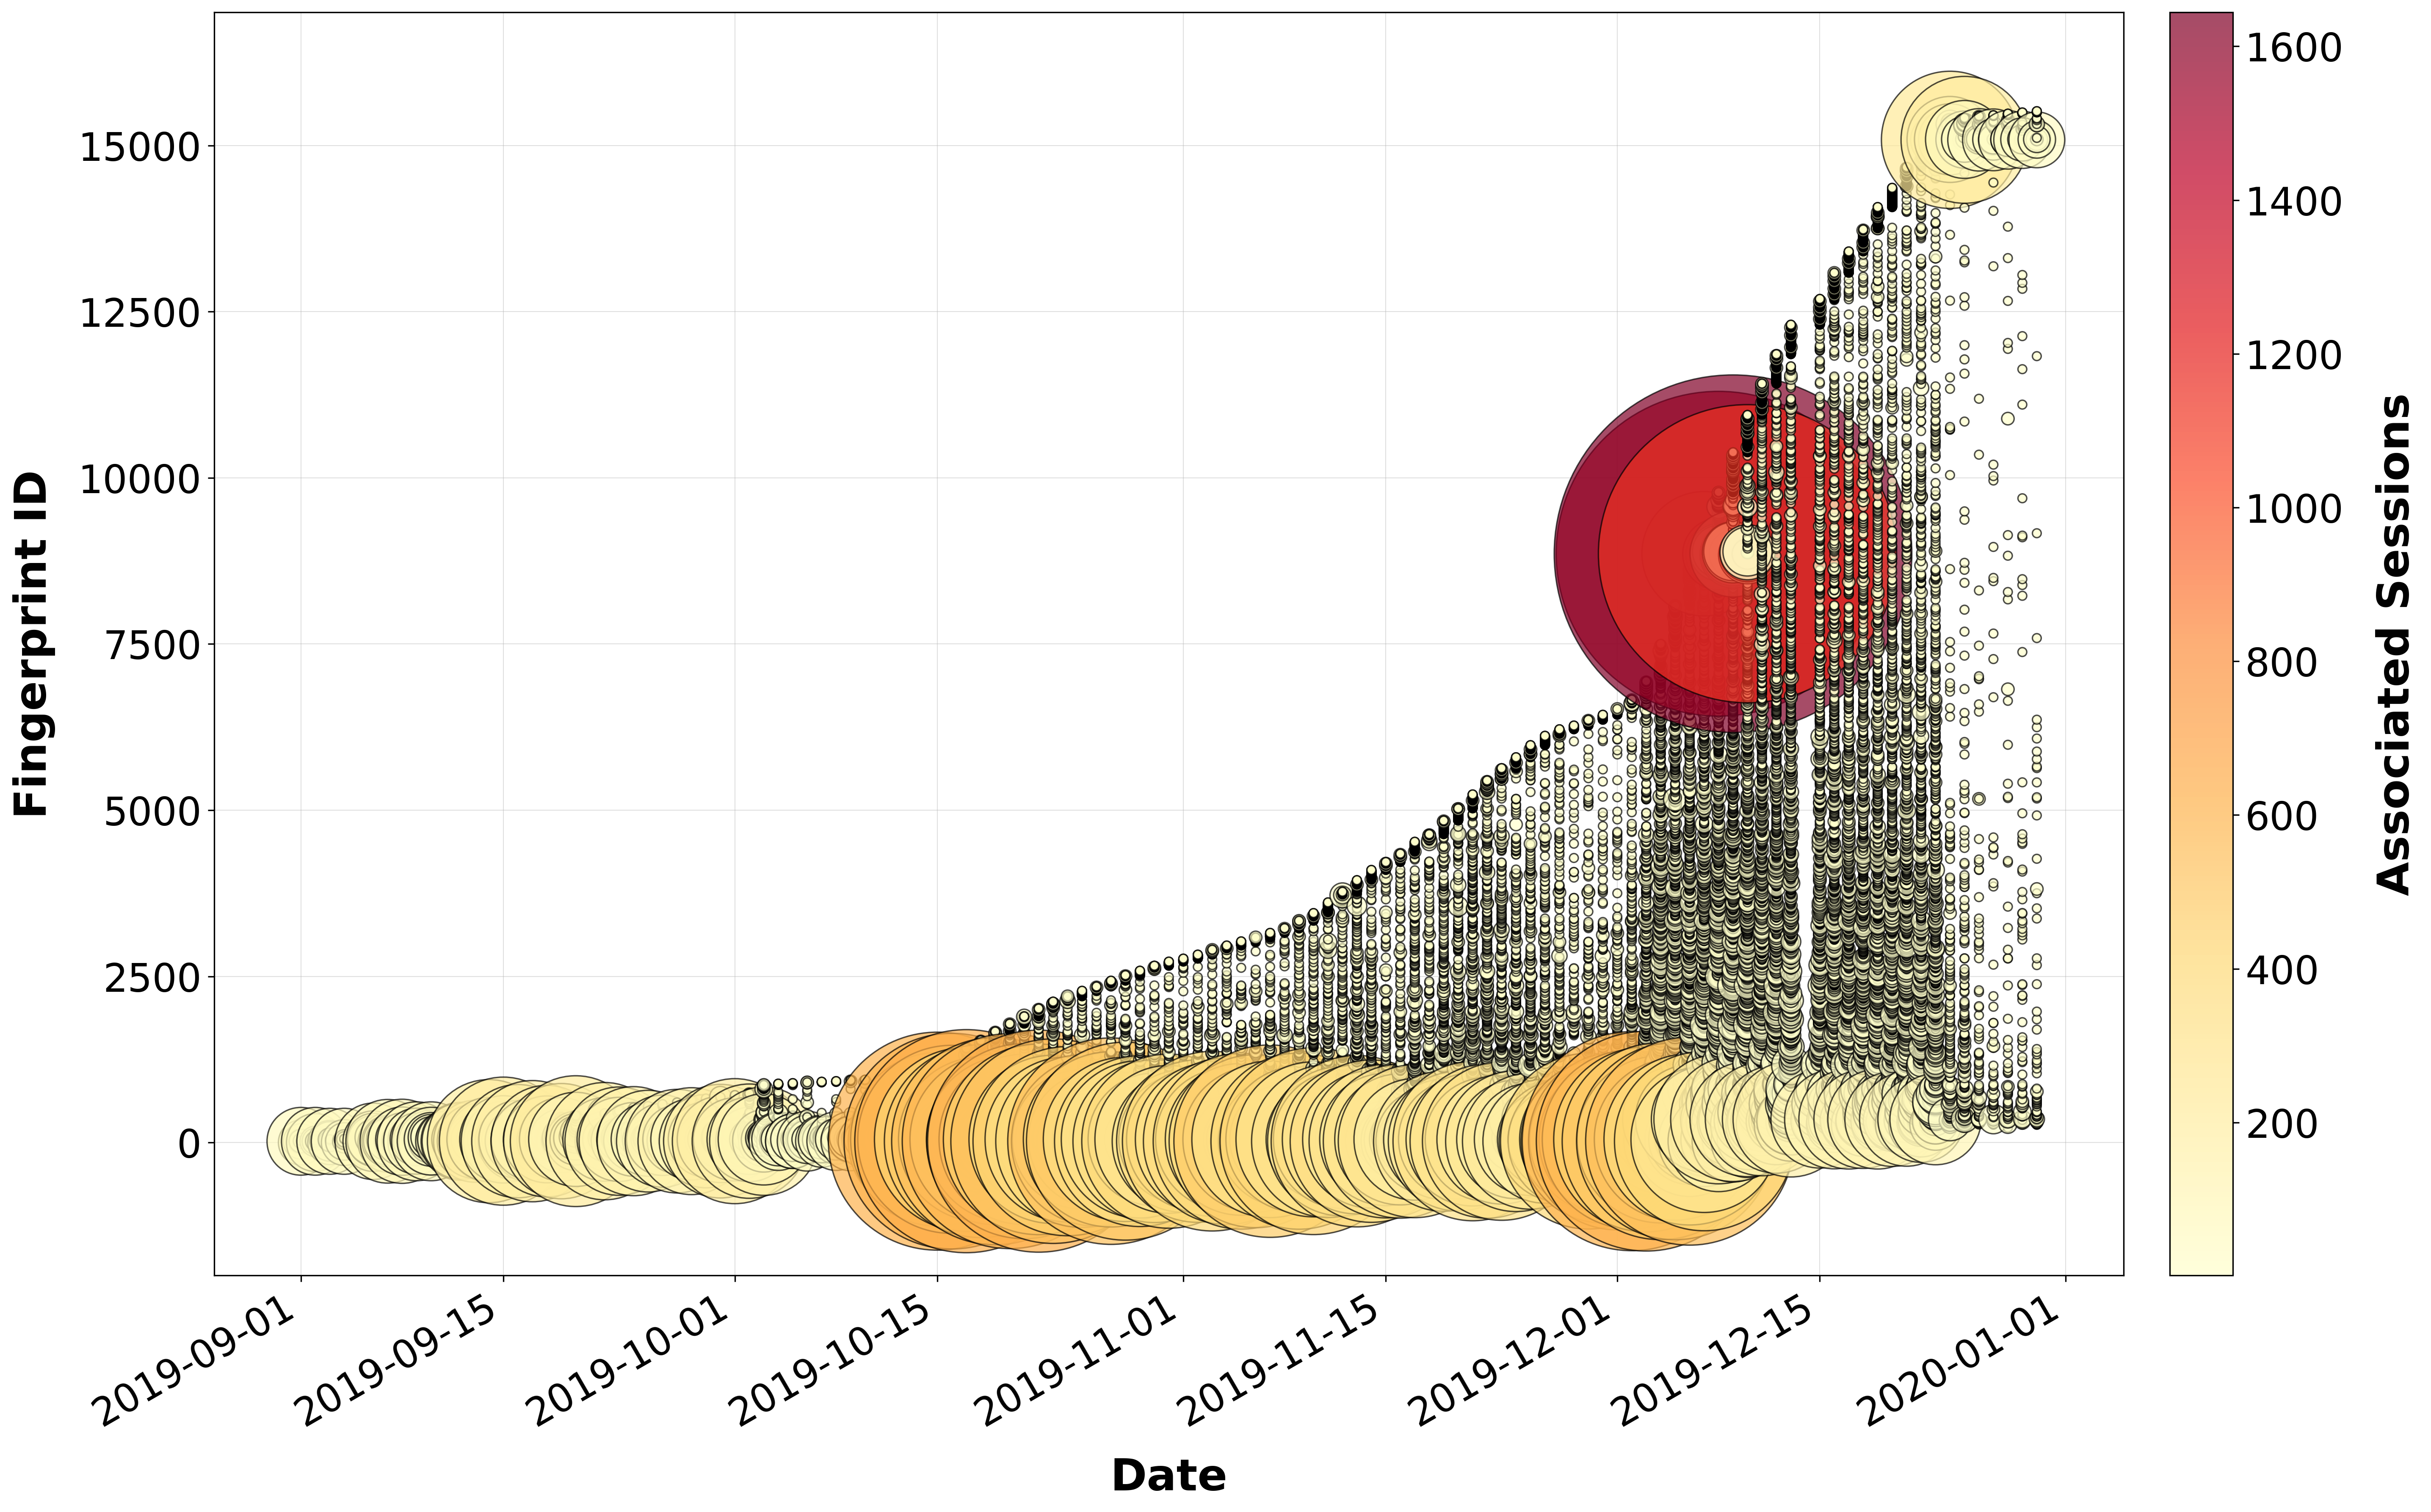
\includegraphics[width=0.9\linewidth]{img/Task4/fingerprint_timeline2.png}
	\caption[Reference architecture schema.]{Reference architecture schema. Only the interfaces represented by a solid line will be standardized in accordance with eIDAS.}
	\label{fig:architectureschema}
\end{figure}

\end{document}
